\documentclass[11pt]{article}

\usepackage[final]{acl}
\usepackage{times}
\usepackage{latexsym}
\usepackage[T1]{fontenc}
\usepackage[utf8]{inputenc}
\usepackage{microtype}
\usepackage{inconsolata}
\usepackage{graphicx}
\usepackage{amsmath}
\usepackage{amssymb}
\usepackage{booktabs}
\usepackage{multirow}

\setlength\titlebox{13\baselineskip}

\title{Does Protecting the Router in Quantized MoE\\
  Improve Accuracy, and How?}

\author{Tomer Alfandary \and Yoav Geva \\
  Tel Aviv University \\
  \texttt{\{tomeralfa13, geva.yoav\}@gmail.com}}

\newcommand{\gold}{\textsc{gold}}
\newcommand{\uniform}{\textsc{uniform}}
\newcommand{\mixed}{\textsc{mixed}}
\newcommand{\placebo}{\textsc{placebo}}
\newcommand{\attn}{\textsc{attention}}

\begin{document}
\maketitle
\begin{abstract}
Mixture-of-Experts (MoE) models spend almost all of their parameters in expert
networks, and only a tiny fraction in the routers that choose them. We ask a
narrow question: in calibration-free, weight-only post-training quantization,
does leaving just those routers in BF16 protect routing and language-model
quality? On OLMoE-1B-7B and Qwen1.5-MoE-A2.7B, at INT8, INT4 and INT3, the
answer is yes for routing. Protecting the routers reduces routing KL and top-1
expert flips relative to quantizing them, with disjoint
bootstrap intervals. A parameter-count-matched placebo does nothing. We
then split the drift that remains between its two possible causes, the error in
the activations reaching the router and the rounding of the router's own
weights, to see which contributes more: the activations dominate at INT8, the
rounded weights at INT4. Router protection is cheap and specific. 
\end{abstract}

\section{Introduction}
\label{sec:intro}

A Mixture-of-Experts layer sends each token through a small linear
\emph{router} and then through only a handful of \emph{experts}
\citep{shazeer2017outrageously,fedus2022switch,jiang2024mixtral}. The experts
are almost the whole model. The routers are not: $0.030\%$ of OLMoE-1B-7B and
$0.021\%$ of Qwen1.5-MoE-A2.7B. Quantizing the experts therefore saves nearly
everything. Quantizing the routers as well can send a token to the wrong
experts.

We test one safeguard, with no calibration: keep every router in BF16 and
quantize every expert. The comparison is a single variable. \uniform{}
quantizes routers and experts at the same INT-$N$ width; \mixed{} quantizes
the same experts and leaves the routers untouched; \gold{} is the BF16
reference. A parameter-count-matched \placebo{} then asks whether protecting
any equally small set of weights would have done as well.

This is not a new proposal. \citet{fu2025eaquant} already run similar experiments and \citet{routequant2026} argue that freezing the
router is not enough. What those papers do not isolate is the
calibration-free, weight-only version of the variable, scored on routing
itself, with a control and a mechanism split. That is the measurement we
report.

Three findings, previewed in Figure~\ref{fig:headline}. First, \mixed{} beats
\uniform{} on routing KL and top-1 expert flips in every model $\times$
bit-width cell we ran. Second, the gain is specific to the routers: the
placebo lands on \uniform{}. Third, we split the drift that remains
between the hidden states arriving at the router and the rounding of the
router's own weights (Section~\ref{sec:attribution}), and find that the hidden
states are the larger source of flips at INT8, while for INT4 the router's own weights are the main cause.

\begin{figure*}[t]
  \centering
  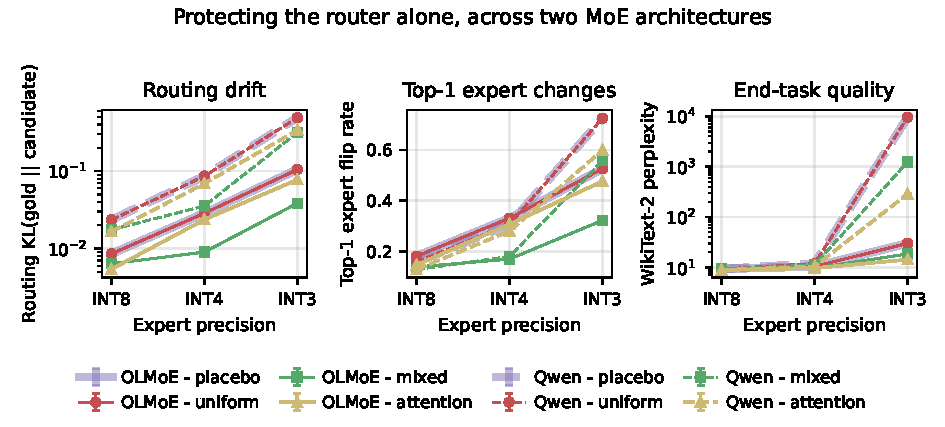
\includegraphics[width=\textwidth]{figures/headline.pdf}
  \caption{Routing KL (left, log scale), top-1 expert flip rate (centre) and
    WikiText-2 perplexity (right, log scale) against expert precision.
    \mixed{} keeps every router in BF16; \uniform{} quantizes the routers
    too; \placebo{} protects a parameter-count-matched non-router module
    instead. Error bars are $95\%$ bootstrap intervals over sequences.
    \placebo{} sits on \uniform{}, that coincidence is the control
    result. The extra series, \attn{}, is a follow-up that also leaves
    attention in BF16 (Section~\ref{sec:results}); it is not a substitute
    for protecting the router.}
  \label{fig:headline}
\end{figure*}

\section{Background}
\label{sec:background}

\paragraph{MoE routing.}
At each MoE layer a linear router maps a hidden state $x\in\mathbb{R}^{d}$
to $E$ logits. The layer keeps the top-$k$ experts and mixes their outputs
with a softmax over those $k$ scores:
\begin{equation}
  y \;=\; \sum_{i\in\mathrm{Top}k(Wx)}
  \mathrm{softmax}(Wx){i}\,E{i}(x).
  \label{eq:moe}
\end{equation}
A flip of the top-1 index, or of the top-$k$ set, changes which parameters
compute $y$. OLMoE uses $E{=}64$, $k{=}8$; Qwen1.5-MoE uses $E{=}60$,
$k{=}4$, plus a shared expert that we do \emph{not} protect
(Section~\ref{sec:method}).

\paragraph{Post-training quantization.}
We use weight-only, per-output-channel symmetric INT-$N$ quantization
through TorchAO \citep{or2025torchao}, with scales taken from the weight
tensor itself. There is no calibration set, no rotation, and no
reconstruction loss. Embeddings and the language-model head stay in BF16 in
every policy. This is a different regime from GPTQ, AWQ, SmoothQuant or
LLM.int8()
\citep{frantar2023gptq,lin2024awq,xiao2023smoothquant,dettmers2022llmint8},
all of which fit something to data.

\paragraph{Metrics.}
Against the \gold{} router we report the KL between full softmaxes
(\emph{routing KL}), the rate at which the top-1 expert changes
(\emph{top-1 flip}), and the Jaccard distance of the top-$k$ sets.
WikiText-2 perplexity \citep{merity2017pointer} is a point estimate over
every scored token; it carries no confidence interval, and the decision
gate does not use it.

\section{Related Work}
\label{sec:related}

\paragraph{Router precision in MoE quantization.}
Protecting the router is already standard practice. EAQuant runs experts at
W4A4 (4-bit integer weights and activations) with the router at W8A8 \citep{fu2025eaquant}. On the same OLMoE
checkpoint we use, their Table~4 holds experts at W3A4 and moves the router
from W3A4 to W8A8; WikiText-2 perplexity falls by $0.32$ and average
zero-shot accuracy rises by about one point. That is a real router-precision
effect, and we do not claim otherwise. It is also confounded in three ways
this paper removes. Every condition moves router \emph{weight and
activation} precision together; the baseline is a calibrated rotation
method; and the most-protected router is W8A8, never a router exempt from
quantization. The table is scored only on end-task metrics, so it cannot
say whether routing itself changed. GEMQ independently notes that routers
are under $0.04\%$ of MoE parameters \citep{deng2026gemq}, which matches
our census.

\paragraph{Repairing routing with data.}
A second line of work treats routing drift as something to fit. VSRAQ adds
value- and structure-alignment losses at 4-bit
\citep{park2026vsraq}. \citet{hyeon2026retrainingfree} argue that
retraining-free compression is not enough and that the router needs
calibration. Both papers are the opposing regime: they spend data on the
router. We spend none.

\paragraph{Whether protection is sufficient.}
The closest work to ours is \emph{Beyond Freezing the Router} by
\citet{routequant2026}, who pair rank-aligned quantization with two
calibration-fitted alignment losses. They argue that freezing the router is
insufficient: quantized expert outputs shift the hidden states
that reach the next layer's router, so a protected router still
misroutes. Their controlled router-precision table on OLMoE
appears to contradict us directly, with an FP16 router slightly
\emph{worse} than a quantized one under W4A4 experts. Their
Table~8 splits that comparison by whether their alignment losses
are active, and on our reading the two branches disagree. Without
the losses, the FP16 router wins on OLMoE and DeepSeek-MoE and
ties on Qwen3-MoE; router quantization overtakes protection only
once a calibration-fitted objective has realigned it. The
disagreement is therefore conditional on calibration rather than
absolute. We occupy the calibration-free branch, where their own
numbers favour protection, and we score it on routing behaviour,
which they report only through end-task metrics, not as KL, flip
rate, or load collapse.

\paragraph{Bit-width sweeps over MoE sub-structures.}
QuantMoE-Bench sweeps precision across attention, experts, block depth and
linear types \emph{inside} experts \citep{li2024quantmoebench}. The router
is not a condition. Its ``gate projection'' analysis is the FFN gate inside
each expert, not the routing gate. MoQE found that expert FFNs tolerate
much lower precision than attention \citep{kim2023moqe}. That fact
motivates a follow-up in Section~\ref{sec:results}, not the main design.

\section{Method}
\label{sec:method}

\paragraph{Three policies, one variable.}
\gold{} is BF16 everywhere. \uniform{} quantizes every linear module at
INT-$N$, including every router. \mixed{} uses the same INT-$N$ policy and
skips the router. Qwen's
\texttt{shared\_expert\_gate} is left quantized, so \mixed{} means the same
thing on both models. Offline inspection of the stored router weights
confirms the single-variable claim: every \mixed{} router is bit-identical
to \gold{} in every layer, and every \uniform{} router sits at the INT-$N$
level ceiling at INT4 and INT3, and well below it at INT8
(Appendix~\ref{sec:appendix-gates}).

\paragraph{A parameter-count-matched control.}
\placebo{} is \uniform{} except that one randomly chosen non-router module,
matched to the total router parameter budget, stays in BF16
(\texttt{placebo\_seed}${=}0$). On OLMoE that module is the layer-14
expert-10 down-projection ($1.000\times$ the budget); on Qwen, the
layer-19 expert-45 down-projection ($0.978\times$). The
control matches parameter count and nothing else. The routers are 16 (24)
small modules read by every token in every layer; the placebo is one expert
down-projection in one layer, on the compute path for $11.4\%$ ($5.0\%$) of
routing tokens. Counting token$\times$layer events, the routers are
exposed about $140\times$ and $477\times$ more. The control rules out
``any high-precision parameters help.''

\paragraph{Four-cell attribution of the residual.}
Even a BF16 router can misroute if the hidden state arriving at it has
already drifted through quantized attention and experts. Table~\ref{tab:fourcell}
crosses gold versus quantized router weights with gold versus
quantized incoming activations. The four logit sets are offline matrix
multiplications on activations captured during the main runs: $X$ stacks
the per-token hidden states $x$ of Equation~\ref{eq:moe} into one matrix,
$W$ is the router weight of that layer, and a cell is
$\mathrm{logits}=XW^{\top}$. Cell C \emph{is} \mixed{}: the same attention and expert
weights as \uniform{}, with no feedback from perturbed routing. Cell D
pairs quantized router weights with those same \mixed{} activations, so it
is \textbf{not} \uniform{}. In a real \uniform{} run a rounded router sends
a token to different experts, those experts write different values into the
residual stream, and every later router therefore sees a different input.
Cell D holds its inputs fixed, so it measures the rounded router weights
alone and omits that feedback. We score every cell against the rebuilt reference A,
and we quote only one share: among tokens flipped by exactly one
mechanism, the fraction flipped by the router's own weights, $B/(B{+}C)$.
The two mechanisms are not additive (Section~\ref{sec:attribution}), so we
do not partition D.

\begin{table}[t]
\centering
\small
\setlength{\tabcolsep}{3pt}
\begin{tabular}{lcc}
\toprule
 & gold $W$ & quantized $W$ \\
\midrule
gold $X$ & A: reference & B: weight error \\
quantized $X$ & C: activation drift & D: both, no feedback \\
 & ($=$\mixed{}) & ($\neq$\uniform{}) \\
\bottomrule
\end{tabular}
\caption{The four-cell design. All four cells are
  $\mathrm{logits}=XW^{\top}$ on captured activations. Metrics are scored
  against cell~A.}
\label{tab:fourcell}
\end{table}

\section{Experiments}
\label{sec:results}

\paragraph{Setup.}
We evaluate OLMoE-1B-7B-0924
\citep{muennighoff2024olmoe} and Qwen1.5-MoE-A2.7B
\citep{qwen2024moe,qwen2023technical} on the WikiText-2 test split
\citep{merity2017pointer}: $288{,}730$ / $299{,}078$ tokens, of which
$288{,}448$ / $298{,}785$ are scored under a $1024$-token window with
stride $1024$. Routing metrics use a seeded subset of $128$ sequences
$\times$ $256$ tokens ($32{,}768$ tokens per layer), with $95\%$
percentile bootstrap intervals from $200$ sequence-level resamples
(\texttt{seed}${=}42$). We sweep INT8, INT4 and INT3. There is no
calibration set. The sweep is WikiText-2 throughout; an INT4 check on C4
is reported below.

\paragraph{Router protection helps, on both architectures.}
Table~\ref{tab:part1} is the main result. \mixed{} beats \uniform{} on
routing KL and top-1 flip rate at every bit-width on both models. The
$95\%$ confidence intervals never overlap
(Tables~\ref{tab:gate} and~\ref{tab:kl-ci}). The effect grows as
precision drops: on OLMoE, routing KL falls from $0.0085$ to $0.0064$ at
INT8, $0.0286$ to $0.0090$ at INT4, and $0.1049$ to $0.0385$ at INT3. Qwen
repeats the pattern. Perplexity moves in the same direction at INT8 and
INT4. Qwen INT3 is saturation, perplexities of $9555$ and $1236$ against a
\gold{} of $7.97$, and we do not treat those ratios as a quality result.
Routing and collapse metrics at INT3 stay in range and remain monotone.

\begin{table*}[t]
\centering
\small
\setlength{\tabcolsep}{4pt}
\begin{tabular}{llcccc}
\toprule
Model & Policy & Bits & PPL & Routing KL & Top-1 flip \\
\midrule
\multirow{7}{*}{OLMoE}
 & \gold{} & BF16 & $8.36$ & $0.0000$ & $0.00\%$ \\
 & \uniform{} / \placebo{} & INT8 & $9.39$ / $9.39$ & $0.0085$ / $0.0085$ & $18.01\%$ / $18.01\%$ \\
 & \mixed{} & INT8 & $9.32$ & $0.0064$ & $13.76\%$ \\
 & \uniform{} / \placebo{} & INT4 & $10.49$ / $10.49$ & $0.0286$ / $0.0286$ & $33.01\%$ / $33.01\%$ \\
 & \mixed{} & INT4 & $9.69$ & $0.0090$ & $16.86\%$ \\
 & \uniform{} / \placebo{} & INT3 & $30.23$ / $30.23$ & $0.1049$ / $0.1049$ & $52.52\%$ / $52.52\%$ \\
 & \mixed{} & INT3 & $18.64$ & $0.0385$ & $32.15\%$ \\
\midrule
\multirow{7}{*}{Qwen}
 & \gold{} & BF16 & $7.97$ & $0.0000$ & $0.00\%$ \\
 & \uniform{} / \placebo{} & INT8 & $9.35$ / $9.35$ & $0.0235$ / $0.0235$ & $15.65\%$ / $15.65\%$ \\
 & \mixed{} & INT8 & $9.28$ & $0.0175$ & $12.75\%$ \\
 & \uniform{} / \placebo{} & INT4 & $12.01$ / $12.01$ & $0.0861$ / $0.0861$ & $30.62\%$ / $30.62\%$ \\
 & \mixed{} & INT4 & $11.24$ & $0.0355$ & $17.90\%$ \\
 & \uniform{} / \placebo{} & INT3 & $9555$ / $9563$ & $0.4901$ / $0.4901$ & $72.48\%$ / $72.48\%$ \\
 & \mixed{} & INT3 & $1236$ & $0.3147$ & $55.69\%$ \\
\bottomrule
\end{tabular}
\caption{Main results. \gold{} is the BF16 upper bound. \placebo{} is
  printed beside \uniform{} because the two agree to several decimals;
  that is the control passing. Top-$k$ Jaccard distance tracks the flip
  rate in every cell (Table~\ref{tab:appendix-jaccard}). Qwen INT3 is
  saturated; perplexity claims in the text use INT8 and INT4 only.}
\label{tab:part1}
\end{table*}

\begin{table*}[t]
\centering
\small
\begin{minipage}[t]{0.48\textwidth}
\centering
\setlength{\tabcolsep}{3pt}
\begin{tabular}{llcc}
\toprule
Model & Bits & \uniform{} & \mixed{} \\
\midrule
OLMoE & INT8 & $18.01_{\,[17.81,18.18]}$ & $13.76_{\,[13.61,13.90]}$ \\
OLMoE & INT4 & $33.01_{\,[32.71,33.31]}$ & $16.86_{\,[16.71,16.99]}$ \\
OLMoE & INT3 & $52.52_{\,[52.21,52.83]}$ & $32.15_{\,[31.86,32.39]}$ \\
Qwen & INT8 & $15.65_{\,[15.47,15.80]}$ & $12.75_{\,[12.58,12.90]}$ \\
Qwen & INT4 & $30.62_{\,[30.44,30.82]}$ & $17.90_{\,[17.69,18.13]}$ \\
Qwen & INT3 & $72.48_{\,[72.11,72.85]}$ & $55.69_{\,[55.41,55.99]}$ \\
\bottomrule
\end{tabular}
\caption{Top-1 flip rate (\%). $95\%$ percentile intervals from $200$
  sequence-level resamples. Every \uniform{}/\mixed{} pair is disjoint.}
\label{tab:gate}
\end{minipage}
\hfill
\begin{minipage}[t]{0.48\textwidth}
\centering
\setlength{\tabcolsep}{3pt}
\begin{tabular}{llcc}
\toprule
Model & Bits & \uniform{} & \mixed{} \\
\midrule
OLMoE & INT8 & $8.54_{\,[8.33,8.76]}$ & $6.36_{\,[6.16,6.55]}$ \\
OLMoE & INT4 & $28.58_{\,[28.10,29.10]}$ & $9.01_{\,[8.73,9.30]}$ \\
OLMoE & INT3 & $104.9_{\,[102.4,107.5]}$ & $38.46_{\,[36.77,40.16]}$ \\
Qwen & INT8 & $23.47_{\,[22.86,24.04]}$ & $17.48_{\,[16.89,18.04]}$ \\
Qwen & INT4 & $86.12_{\,[84.86,87.38]}$ & $35.49_{\,[34.59,36.46]}$ \\
Qwen & INT3 & $490.1_{\,[484.6,496.5]}$ & $314.7_{\,[310.6,319.0]}$ \\
\bottomrule
\end{tabular}
\caption{Routing KL $(\times 10^{-3})$, same intervals. Reductions are
  $25.5\%$, $68.5\%$, $63.3\%$ on OLMoE and $25.5\%$, $58.8\%$, $35.8\%$
  on Qwen.}
\label{tab:kl-ci}
\end{minipage}
\end{table*}

\paragraph{The effect is router-specific.}
\placebo{} reproduces \uniform{} on every reported metric, at all three
bit-widths, on both models (Table~\ref{tab:part1}). Protecting a random
$0.03\%$ of parameters is not what helps.

\paragraph{Follow-up: keeping attention in BF16.}
Figure~\ref{fig:headline} includes a later series, \attn{}, that leaves
every attention projection in BF16 and keeps the routers quantized
\citep{kim2023moqe}. Attention is $3.88\%$ of OLMoE and $2.81\%$ of Qwen,
about $128\times$ the router budget, so a better perplexity number is the
expected tradeoff, not a rival result. On routing KL it recovers only
part of \mixed{}'s gain at INT4 and INT3, and more than all of it at INT8
(Table~\ref{tab:appendix-attnkl}), which is the attribution ranking of
Section~\ref{sec:attribution} appearing as a policy. Specificity is
\placebo{}'s job, not \attn{}'s. We expect leaving both the routers
\emph{and} attention in BF16 to improve further still, but that is a
different tradeoff, and we leave it to a paper whose purpose is that mix.

\paragraph{Expert collapse, resolved per layer.}
Pooled usage entropy sits near $0.99$ in every run and hides the only
real collapse in the sweep. Counted per layer, a slot is starved when
that expert takes under a tenth of an even share. Qwen INT3 under
\uniform{} starves $222$ of $1{,}440$ slots and leaves a fully unused
expert in five layers; \mixed{} starves $55$ and leaves none unused
(Figure~\ref{fig:collapse}, Table~\ref{tab:collapse}).

On OLMoE nothing collapses. The unquantized model already has $17$
specialists below the line; rounding flattens load and lifts them over
it, so the starved count falls as routing degrades. That is not a
benefit. \mixed{} stays nearer \gold{} than \uniform{} does. These are
single-seed counts with no interval, so we rest on the Qwen gap, a factor
of four, and not on a few OLMoE slots.

\begin{figure}[t]
  \centering
  \includegraphics[width=\columnwidth,page=3,trim={0 0 0 27},clip]{figures/collapse_qwen.pdf}
  \caption{Starved experts by layer on Qwen at INT3, the one cell where
    collapse occurs. A slot is starved when an expert receives under a
    tenth of its even share in its own layer. \uniform{} and \placebo{}
    coincide, so the \uniform{} line is hidden beneath the \placebo{} one.
    \mixed{} keeps every expert alive, as does the later \attn{} series.
    Damage concentrates in the mid-to-late layers, which pooled entropy
    averaged away. The OLMoE counterpart is flat at every depth and
    bit-width.}
  \label{fig:collapse}
\end{figure}

\paragraph{Where the sweep stops being informative.}
Qwen INT3 is destroyed under every quantized policy (top-1 agreement with
\gold{} output falls to $6.6\%$ / $12.8\%$). The ranking among ruined
models is not a quality claim. We use INT3 for routing and collapse, which
stay finite and ordered, and we make perplexity claims at INT8 and INT4.

\paragraph{A second corpus reproduces the INT4 result.}
To test whether the routing effect is a property of WikiText-2, we re-ran
the INT4 cell on both models on C4 \citep{raffel2020t5}, holding seed,
routing-subset shape and gates fixed. The ordering repeats on both
architectures, including the attribution share
(Appendix~\ref{sec:appendix-c4}). INT8 and INT3 were not repeated. 

\section{Attribution Analysis}
\label{sec:attribution}

\paragraph{The rebuild reproduces the runs.}
Cell A, rebuilt from stored activations and weights, matches the routing
decisions the \gold{} run recorded at $99.66\%$ mean top-1 agreement on
OLMoE (worst layer $99.46\%$) and $99.37\%$ on Qwen (worst layer
$98.49\%$). That floor is reconstruction noise: fp16-stored activations,
recomputed in CPU fp32, against a BF16 GPU forward pass. Every difference
in Table~\ref{tab:attribution} is well above it. Cell C also matches the
\mixed{} flip rates measured in Part~1 (OLMoE INT4: $16.62\%$ rebuilt vs.\
$16.86\%$ recorded). On top-1 flips, cell D falls a little short of
\uniform{}, as it must: OLMoE INT3 is $50.01\%$ versus $52.52\%$; Qwen INT3
is $68.58\%$ versus $72.48\%$. The gap is the routing-feedback term that D
omits. Routing KL orders the same way at INT4 and INT3, but not at INT8,
where D slightly exceeds \uniform{} on both models ($0.0091$ versus
$0.0085$ on OLMoE, $0.0260$ versus $0.0235$ on Qwen). INT8 is where the
measured quantity is smallest and therefore closest to the rebuild's
reconstruction floor, so we read that inversion as reconstruction noise
rather than as a feedback term that has changed sign.

\paragraph{The dominant mechanism reverses between INT8 and INT4.}
Of the flips caused by exactly one mechanism, the router's own weights
account for $43.4\%$ / $40.3\%$ at INT8 (OLMoE / Qwen) and $62.2\%$ /
$58.0\%$ at INT4 (Table~\ref{tab:attribution}). Above half, router
protection removes the larger source. That crossover is the same on both
architectures, and it is the same on routing KL
(Table~\ref{tab:appendix-kl}). At INT8 the cheap safeguard is fighting
the smaller fire. At INT4 it is fighting the larger one. We do not read
Qwen INT3 ($45.4\%$) as activation dominance returning: that cell is the
saturated regime of Section~\ref{sec:results}.

\paragraph{What the share does not say.}
The interaction residual $1-B/D-C/D$ is large and negative everywhere
($-36\%$ to $-51\%$). The two mechanisms flip overlapping token sets: a
token that either source alone would have flipped is counted once in D
and twice across B and C. $B/D$ and $C/D$ are therefore not shares of
anything that sums to $100\%$, and we do not write an
``$X\%$ / $(100{-}X)\%$'' split.

\begin{table}[t]
\centering
\small
\setlength{\tabcolsep}{3pt}
\begin{tabular}{llcccc}
\toprule
Model & Bits & B & C & D & $B/(B{+}C)$ \\
\midrule
OLMoE & INT8 & $10.4$ & $13.5$ & $17.5$ & $43.4_{\,[42.7,44.1]}$ \\
OLMoE & INT4 & $27.4$ & $16.6$ & $31.4$ & $62.2_{\,[61.7,62.8]}$ \\
OLMoE & INT3 & $43.8$ & $31.7$ & $50.0$ & $58.0_{\,[57.6,58.4]}$ \\
Qwen & INT8 & $8.8$ & $13.0$ & $15.7$ & $40.3_{\,[39.8,40.9]}$ \\
Qwen & INT4 & $25.0$ & $18.1$ & $30.3$ & $58.0_{\,[57.5,58.5]}$ \\
Qwen & INT3$^{*}$ & $45.8$ & $55.1$ & $68.6$ & $45.4_{\,[45.1,45.6]}$ \\
\bottomrule
\end{tabular}
\caption{Attribution of top-1 flips (\%), $10{,}000$ bootstrap
  replicates. B, C and D follow Table~\ref{tab:fourcell}. $B/(B{+}C)$ is
  the share of single-mechanism flips due to the router's own weights.
  The residual $1-B/D-C/D$ is $-36\%$ to $-51\%$ in every row, so the
  shares of D do not partition the drift. $^{*}$Saturated.}
\label{tab:attribution}
\end{table}

\section{Discussion}
\label{sec:discussion}

\paragraph{Necessary but not sufficient.}
Leaving the routers in BF16 is a free, specific way to keep routing close
to the unquantized model. It is free because the routers are $0.02\%$ to
$0.03\%$ of the weights. It is specific because a parameter-count-matched
placebo does nothing. It is not sufficient for end-task quality, because a
large share of the remaining routing error, and most of the perplexity
error, comes from the residual stream, not from the router matrix. A later
run that also protects attention improves perplexity, as expected from its
size; that is extra precision on top of the router question, not an
alternative answer to it.

\paragraph{Adjudicating the disagreement.}
The literature looks inconsistent only if calibration is ignored.
EAQuant's ablation shows that a more precise router helps, on a calibrated
W+A baseline, scored on perplexity \citep{fu2025eaquant}. \citeauthor{routequant2026}'s
headline says freezing the router is not enough, and their own no-alignment
split says the opposite in the calibration-free case
\citep{routequant2026}. We measure that case on routing. Protecting the
router is the right default when no data will be spent on it. It does not
replace a method that realigns routing with calibration
\citep{park2026vsraq,hyeon2026retrainingfree,routequant2026}.

\section{Limitations}
\label{sec:limitations}

The reported magnitudes are in-domain on WikiText-2; the C4 check is
INT4 only. Perplexity is a point estimate and carries no interval, and the
expert collapse counts of Section~\ref{sec:results} are single-seed draws
with no interval either. \placebo{} is a single draw, matched on parameter
count rather than on activation exposure, and every run uses one seed.
``Cheap'' is a claim about parameter share and nothing else. We do not
report memory or speed: these GPUs unpack the integer weights back to
floats before multiplying, so a savings number would not be a real
integer-kernel result, and a BF16 island inside an otherwise INT-$N$ graph
can force dtype conversions that a parameter count does not capture. That
was not the question we set out to answer. DeepSeek-style routers, whose
gate is a bare parameter rather than an \texttt{nn.Linear}
\citep{dai2024deepseekmoe}, perform differently, and we did not evaluate
their behaviour.

\section{Conclusion}
\label{sec:conclusion}

We asked whether, under calibration-free weight-only quantization, leaving
only the MoE routers in BF16 reduces routing drift and perplexity loss.
It reduces routing drift, cheaply and specifically, on two architectures
and three bit-widths. The residual error switches source between INT8 and
INT4, so a full-precision receptionist still misroutes if the chart on
her desk is already wrong. Spending more precision on attention as well
is a separate, larger tradeoff, in addition, not instead.

\section*{AI Disclosure and Reflection}
As in earlier work for this course, we used AI assistants as a third
partner, with us as the orchestrators throughout: every step was
specified, reviewed and accepted by us. Gemini supported the literature
search and the brainstorming that narrowed our proposal to the
calibration-free, weight-only version of the router question; we went through every cited paper ourselves. Once the design was fixed we moved to
Cursor (mainly Grok 4.6 and Opus 5), working step by step
through the repository, the quantization and evaluation code, the
analysis scripts and the tests. We also used assistance to structure
and word this report and to pressure-test which claims the tables
support. Every number in every table was transcribed from the run
artifacts and checked against the corresponding JSON. The research
question, the experimental matrix, the decision to treat the four-cell
rebuild as a mechanism analysis rather than a fallback, the controls,
and the interpretation are ours; the tools assisted, they did not
decide.

On reflection, the assistance was most useful where the work was
mechanical and checkable, such as the policy construction and the offline
analyses, which we could hold to tests we had read. It was least useful
where the work was generative. Draft prose reliably reached for more
confidence than the tables supported, and several claims in earlier
versions of this report had to be narrowed or cut once we compared them
against the run artifacts, including a novelty claim that a closer reading
of EAQuant's ablation table did not survive. The habit that made the
difference was treating every generated sentence about a number as a
hypothesis to check rather than a result to keep.

\bibliography{custom}

\appendix

\section{Experimental setup}
\label{sec:appendix-setup}

\paragraph{Models.}
Table~\ref{tab:params} records the two checkpoints. Both expose the router
as \texttt{nn.Linear} named \texttt{mlp.gate}. We pin
\texttt{transformers} to $4.x$ so experts remain individual linear modules
rather than a fused 3D stack, which a walker that only swaps
\texttt{nn.Linear} would silently skip.

\begin{table}[t]
\centering
\small
\setlength{\tabcolsep}{4pt}
\begin{tabular}{lcc}
\toprule
 & OLMoE & Qwen \\
\midrule
Layers / experts / $k$ & $16$ / $64$ / $8$ & $24$ / $60$ / $4$ \\
Total params & $6.92$B & $14.32$B \\
Router params & $2.10$M & $2.95$M \\
Router share & $0.0303\%$ & $0.0206\%$ \\
\bottomrule
\end{tabular}
\caption{Architectures, from \texttt{inspect\_model.py}.
  Checkpoints: \texttt{OLMoE-1B-7B-0924}
  \citep{muennighoff2024olmoe} and \texttt{Qwen1.5-MoE-A2.7B}
  \citep{qwen2024moe,qwen2023technical}.}
\label{tab:params}
\end{table}

\paragraph{Data and protocol.}
WikiText-2 raw test, documents joined with a blank line and tokenized as
one stream. There is no train/test leakage: scales come from the weights,
never from activations, and no hyperparameter is selected on the
evaluation tokens. Routing metrics and perplexity share that stream; they
are not independent confirmations of the same effect. The routing subset
is \texttt{default\_rng(42).choice} over disjoint $256$-token blocks.
Router inputs for attribution are stored every eighth token.

\paragraph{Hardware and reproducibility.}
Runs used NVIDIA GeForce RTX 2080 Ti cards (compute $7.5$), three for
OLMoE and five for Qwen, with \texttt{torch} $2.9.1$,
\texttt{transformers} $4.57.6$ and \texttt{torchao} $0.17.0$
\citep{or2025torchao,wolf2020transformers}. Every results file records
the git commit, package versions, GPU type and a SHA-256 fingerprint of
the token ids. A candidate whose corpus, seed or layout disagrees with
\gold{} is rejected rather than scored.

\paragraph{Deviations from the approved proposal.}
The proposal named \texttt{Qwen/Qwen2.5-MoE-1.4B-A14B}, which does not
exist and is internally contradictory. We substituted OLMoE-1B-7B, one of
the three models EAQuant benchmarks \citep{fu2025eaquant}, and
Qwen1.5-MoE-A2.7B as a second architecture. We swept INT8/4/3 rather than
INT8 alone, because INT8 is nearly lossless and would have left the
comparison inside the noise. The proposal named WikiText-2 and C4; the
sweep is WikiText-2 and C4 enters as the INT4 check of
Appendix~\ref{sec:appendix-c4}. Part~2
was described as a fallback for a null Part~1; Part~1 came out positive
and we ran the attribution anyway, as a mechanism analysis. The
proposal's contingency of scaling routing scores by activation size was
not built.

\section{Correctness gates and offline verification}
\label{sec:appendix-gates}

Every claim in the paper rests on \mixed{} and \uniform{} differing in the
routers and in nothing else. Rather than trust the quantizer's own
bookkeeping, we re-derive that from the artifacts each run stored.
Table~\ref{tab:appendix-gates} counts the modules each policy quantized,
Table~\ref{tab:appendix-verification} inspects the stored router weights
channel by channel, and Table~\ref{tab:appendix-placebo} records what the
\placebo{} draw actually protected.

\begin{table}[t]
\centering
\small
\setlength{\tabcolsep}{4pt}
\begin{tabular}{lrr}
\toprule
Policy & OLMoE & Qwen \\
\midrule
\gold{} & $0$ & $0$ \\
\uniform{} & $3152$ & $4536$ \\
\mixed{} & $3136$ & $4512$ \\
\placebo{} & $3151$ & $4535$ \\
\attn{} & $3088$ & $4440$ \\
\bottomrule
\end{tabular}
\caption{Modules quantized per policy, identical at every bit-width.
  \mixed{} quantizes exactly $16$ (resp.\ $24$) fewer modules than
  \uniform{}, and those modules are the routers. \placebo{} spares one
  extra module. The \attn{} follow-up, listed for completeness, spares
  $64$ (resp.\ $96$) attention projections and keeps every router
  quantized. \gold{} self-comparison is exactly zero KL and zero flips
  on both models.}
\label{tab:appendix-gates}
\end{table}

\begin{table}[t]
\centering
\footnotesize
\setlength{\tabcolsep}{3pt}
\begin{tabular}{llccc}
\toprule
Model & Run & Lev. & Cap & $=$~\gold{} \\
\midrule
OLMoE & \gold{} / \mixed{} & $1161$ & n/a & $16/16$ \\
OLMoE & unif./plac.\ INT8 & $60$ & $256$ & $0/16$ \\
OLMoE & INT4 quantized & $16$ & $16$ & $0/16$ \\
OLMoE & INT3 quantized & $8$ & $8$ & $0/16$ \\
Qwen & \gold{} / \mixed{} & $1107$ & n/a & $24/24$ \\
Qwen & unif./plac.\ INT8 & $46$ & $256$ & $0/24$ \\
Qwen & INT4 quantized & $16$ & $16$ & $0/24$ \\
Qwen & INT3 quantized & $8$ & $8$ & $0/24$ \\
\bottomrule
\end{tabular}
\caption{Offline bit-identity check on the dequantized router weights each
  run stored. \textbf{Levels} is the largest number of distinct values in
  any output channel; \textbf{Cap} is the ceiling $2^{N}$ that per-channel
  symmetric INT-$N$ allows, which does not apply to a router left in BF16.
  INT8 sits far below its cap through occupancy rather than range: the
  per-channel scale is fixed by that channel's largest weight, and the
  remaining weights lie well inside the interval that outlier defines, so
  they land on a narrow band of codes around zero and most of the $256$
  available codes are never the nearest code to any weight. The emptiest
  channel uses only $16$ levels on OLMoE and $11$ on Qwen. All listed runs
  pass. \texttt{scripts/verify\_offline.py}.}
\label{tab:appendix-verification}
\end{table}

\begin{table}[t]
\centering
\small
\setlength{\tabcolsep}{4pt}
\begin{tabular}{lcc}
\toprule
 & OLMoE & Qwen \\
\midrule
Module & L14 E10 & L19 E45 \\
 & \texttt{down\_proj} & \texttt{down\_proj} \\
Params vs.\ budget & $1.000\times$ & $0.978\times$ \\
Tokens on path & $11.43\%$ & $5.04\%$ \\
Exposure gap & $140\times$ & $477\times$ \\
\bottomrule
\end{tabular}
\caption{What \placebo{} protected at \texttt{placebo\_seed}${=}0$. One
  expert down-projection per model, re-derived from a meta-device
  skeleton. The selection rule stops once the accumulated module is
  within $25\%$ of the router budget; on both checkpoints the first
  eligible draw already is.}
\label{tab:appendix-placebo}
\end{table}

\section{Expert collapse: per-layer detail}
\label{sec:appendix-collapse}

The counts behind Figure~\ref{fig:collapse}. Pooling expert usage across
layers cancels per-layer imbalance and reports nothing, so every number
here is resolved within its own layer and then summed.

\begin{table}[t]
\centering
\footnotesize
\setlength{\tabcolsep}{3pt}
\begin{tabular}{llccc}
\toprule
Model & Policy & Starved & Unused & KL \\
\midrule
OLMoE & \gold{} & $17/1024$ & $0$ & $0.131$ \\
OLMoE & \uniform{} INT3 & $6/1024$ & $0$ & $0.163$ \\
OLMoE & \mixed{} INT3 & $9/1024$ & $0$ & $0.141$ \\
OLMoE & \attn{} INT3 & $8/1024$ & $0$ & $0.142$ \\
Qwen & \gold{} & $0/1440$ & $0$ & $0.047$ \\
Qwen & \uniform{} INT3 & $222/1440$ & $5$ & $0.572$ \\
Qwen & \mixed{} INT3 & $55/1440$ & $0$ & $0.269$ \\
Qwen & \placebo{} INT3 & $220/1440$ & $5$ & $0.572$ \\
Qwen & \attn{} INT3 & $74/1440$ & $0$ & $0.346$ \\
\bottomrule
\end{tabular}
\caption{Expert collapse, resolved per layer. A slot is starved when an
  expert receives under a tenth of its fair share in its own layer.
  Starved counts use all $32{,}768$ routing tokens; load KL is rebuilt
  from the strided capture, with \gold{} measured on the same positions.
  OLMoE does not collapse; Qwen INT3 does, and \mixed{} mitigates it.}
\label{tab:collapse}
\end{table}

\section{Additional policy comparisons}
\label{sec:appendix-part1}

Two policy-level views that the main text refers to but does not have room
to print. Table~\ref{tab:appendix-jaccard} gives the top-$k$ Jaccard
distance behind the flip rates in Table~\ref{tab:part1}, and
Table~\ref{tab:appendix-attnkl} gives the routing KL of the \attn{}
follow-up beside \uniform{} and \mixed{}, which is the comparison the
recovery percentages in Section~\ref{sec:results} are computed from.

\begin{table}[t]
\centering
\small
\setlength{\tabcolsep}{4pt}
\begin{tabular}{llccc}
\toprule
Model & Bits & \uniform{} & \mixed{} & \attn{} \\
\midrule
OLMoE & INT8 & $0.145$ & $0.128$ & $0.105$ \\
OLMoE & INT4 & $0.236$ & $0.149$ & $0.206$ \\
OLMoE & INT3 & $0.434$ & $0.277$ & $0.363$ \\
Qwen & INT8 & $0.212$ & $0.185$ & $0.170$ \\
Qwen & INT4 & $0.356$ & $0.244$ & $0.321$ \\
Qwen & INT3 & $0.744$ & $0.617$ & $0.635$ \\
\bottomrule
\end{tabular}
\caption{Top-$k$ Jaccard distance from the \gold{} selected-expert set.
  \gold{} is $0$ by construction. The ordering matches the top-1 flip
  rate. The \attn{} column is the follow-up series from
  Figure~\ref{fig:headline}.}
\label{tab:appendix-jaccard}
\end{table}

\begin{table}[t]
\centering
\footnotesize
\setlength{\tabcolsep}{3pt}
\begin{tabular}{llcccc}
\toprule
Model & Bits & \uniform{} & \mixed{} & \attn{} & Rec. \\
\midrule
OLMoE & INT8 & $0.0085$ & $0.0064$ & $0.0054$ & $144\%$ \\
OLMoE & INT4 & $0.0286$ & $0.0090$ & $0.0237$ & $25\%$ \\
OLMoE & INT3 & $0.1049$ & $0.0385$ & $0.0777$ & $41\%$ \\
Qwen & INT8 & $0.0235$ & $0.0175$ & $0.0165$ & $117\%$ \\
Qwen & INT4 & $0.0861$ & $0.0355$ & $0.0691$ & $34\%$ \\
Qwen & INT3$^{*}$ & $0.4901$ & $0.3147$ & $0.3380$ & $87\%$ \\
\bottomrule
\end{tabular}
\caption{Routing KL for the \attn{} follow-up beside the two main
  policies. \textbf{Rec.} is the fraction of \mixed{}'s reduction that
  \attn{} recovers, $(\uniform{}-\attn{})/(\uniform{}-\mixed{})$, and is
  the quantity quoted in Section~\ref{sec:results}. Values above $100\%$
  mean \attn{} reached a lower routing KL than \mixed{}, which happens
  only at INT8, where Table~\ref{tab:attribution} puts the larger share of
  single-mechanism flips on the incoming activations rather than on the
  router's own weights. $^{*}$Saturated.}
\label{tab:appendix-attnkl}
\end{table}

\section{Attribution: mechanism detail}
\label{sec:appendix-attribution}

Table~\ref{tab:attribution} scores the four-cell rebuild on top-1 flips.
Routing KL is the second metric we can score it on, and it is reported here
to show that the INT8-to-INT4 crossover is not an artifact of thresholding
a continuous drift at the top-1 index.

\begin{table}[t]
\centering
\small
\setlength{\tabcolsep}{4pt}
\begin{tabular}{llccc}
\toprule
Model & Bits & B & C & D \\
\midrule
OLMoE & INT8 & $0.0018$ & $0.0073$ & $0.0091$ \\
OLMoE & INT4 & $0.0175$ & $0.0099$ & $0.0272$ \\
OLMoE & INT3 & $0.0586$ & $0.0393$ & $0.0929$ \\
Qwen & INT8 & $0.0053$ & $0.0207$ & $0.0260$ \\
Qwen & INT4 & $0.0444$ & $0.0387$ & $0.0836$ \\
Qwen & INT3 & $0.1666$ & $0.3145$ & $0.4540$ \\
\bottomrule
\end{tabular}
\caption{Routing KL by mechanism. The INT8-to-INT4 crossover is the same
  as in Table~\ref{tab:attribution}: B $<$ C at INT8 and B $>$ C at INT4
  on both models.}
\label{tab:appendix-kl}
\end{table}

\section{The C4 check in full}
\label{sec:appendix-c4}

Table~\ref{tab:appendix-c4} gives the INT4 cell on both corpora. The C4
runs use \texttt{configs/olmoe\_c4.yaml} and \texttt{configs/qwen\_c4.yaml}:
same seed, routing-subset shape and gates as WikiText-2. One English
validation shard yields $481{,}220$ / $469{,}449$ scored tokens against
$288{,}448$ / $298{,}785$ on WikiText-2. Perplexity is comparable within a
column, not across columns.

\begin{table}[t]
\centering
\small
\setlength{\tabcolsep}{4pt}
\begin{tabular}{llcc}
\toprule
 & INT4 & WikiText-2 & C4 \\
\midrule
\multirow{8}{*}{OLMoE}
 & \gold{} PPL & $8.36$ & $12.29$ \\
 & \uniform{} PPL & $10.49$ & $14.13$ \\
 & \mixed{} PPL & $9.69$ & $13.45$ \\
 & \uniform{} routing KL & $0.0286$ & $0.0273$ \\
 & \mixed{} routing KL & $0.0090$ & $0.0083$ \\
 & \uniform{} top-1 flip & $33.01\%$ & $33.95\%$ \\
 & \mixed{} top-1 flip & $16.86\%$ & $17.00\%$ \\
 & $B/(B{+}C)$ & $62.2\%$ & $63.0\%$ \\
\midrule
\multirow{8}{*}{Qwen}
 & \gold{} PPL & $7.97$ & $10.36$ \\
 & \uniform{} PPL & $12.01$ & $16.00$ \\
 & \mixed{} PPL & $11.24$ & $14.85$ \\
 & \uniform{} routing KL & $0.0861$ & $0.0737$ \\
 & \mixed{} routing KL & $0.0355$ & $0.0272$ \\
 & \uniform{} top-1 flip & $30.62\%$ & $30.03\%$ \\
 & \mixed{} top-1 flip & $17.90\%$ & $16.57\%$ \\
 & $B/(B{+}C)$ & $58.0\%$ & $60.2\%$ \\
\bottomrule
\end{tabular}
\caption{The INT4 cell on both corpora. Orderings survive the corpus
  change. Perplexities are not comparable across columns.}
\label{tab:appendix-c4}
\end{table}

\section{Reproduction}
\label{sec:appendix-repro}

The accompanying repository builds the policies as torchao
\texttt{FqnToConfig} dictionaries, runs them through a shared evaluation
loop, and refuses to score a candidate whose token fingerprint, topology
or router-quantization audit fails. Offline analyses
(\texttt{scripts/analyze.py}, \texttt{attribute.py},
\texttt{collapse.py}, \texttt{verify\_offline.py}) read only the stored artifacts and need no
GPU. The main sweep is:

\begin{verbatim}
python scripts/run.py \
  --config configs/olmoe.yaml \
  --policies gold uniform mixed placebo \
  --bits 8 4 3
python scripts/analyze.py \
  --results-dir results/olmoe
\end{verbatim}

\noindent Add \texttt{attention} to \texttt{--policies} for the
follow-up series in Figure~\ref{fig:headline}.

\noindent Substitute \texttt{configs/qwen.yaml} for the second
architecture. Tests (\texttt{pytest}) cover policy construction, metric
identities, the four-cell rebuild and the registry collisions that would
silently protect the wrong module.

\end{document}